
\documentclass[sigchi]{acmart}

\settopmatter{printacmref=false, printccs=true, printfolios=true}
%%
%% \BibTeX command to typeset BibTeX logo in the docs
\AtBeginDocument{%
  \providecommand\BibTeX{{%
    \normalfont B\kern-0.5em{\scshape i\kern-0.25em b}\kern-0.8em\TeX}}}

%% Rights management information.  This information is sent to you
%% when you complete the rights form.  These commands have SAMPLE
%% values in them; it is your responsibility as an author to replace
%% the commands and values with those provided to you when you
%% complete the rights form.
\setcopyright{none}
%\copyrightyear{none}
\acmYear{2021}
\acmDOI{}

%% These commands are for a PROCEEDINGS abstract or paper.
\acmConference[Technical Report]{May}{{\today}}{Cologne, Germany}
\acmBooktitle{}
\acmPrice{}
\acmISBN{}

\usepackage{subfig}
\usepackage[english, german]{babel}
\begin{document}

\title{The impact of the avatar representation on team trust and effectiveness in a shared virtual environment.}

\author{Hannes Hinrichs}
\email{hhinrich@smail.th-koeln.de}
\affiliation{%
  \institution{TH-Köln}
  \city{Cologne}
  \country{Germany}
}

\begin{abstract}
The goal of this work is to find out if different avatar representations have an impact on the formed trust and effectiveness of a team. The first question here is whether an inverse-kinematic human-like representation or an abstract non-human-like representation is more effective in generating trust in a newly formed virtual team. The second question addresses whether the trust formed by the different representations influences the effectiveness of the virtual team. To answer these questions, a quantitative study was conducted in which different participants in a three-person team performed a collaborative task in a shared virtual environment. No significant differences in effectiveness were found between the teams. The results of the study also show that in the threeperson team significantly more trust was built with non humanlike avatars. Furthermore, with non-human-like avatars there was a significant relationship between the cognitive trust formed and teameffectiveness. This means that the simplicity of a non-human-like avatar in a newly formed team in a shared virtual environment can be effective in creating a trusting work atmosphere.
\end{abstract}

\keywords{Virtual-Reality, Trust, Team formation, virtual Team, Avatar}

%% A "teaser" image appears between the author and affiliation
%% information and the body of the document, and typically spans the
%% page.
\begin{teaserfigure}
  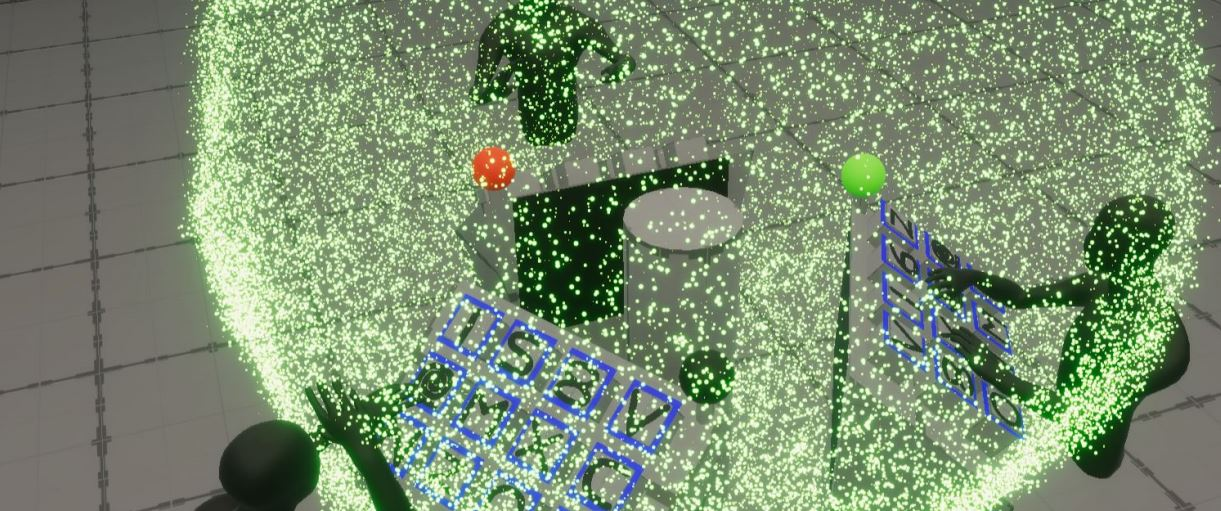
\includegraphics[width=\textwidth]{Abbildungen/RoundSuccsessful2}
  \caption{This figure represents the developed Shared-Virual-Environment infront of there Podests. A green sphere appears clearly visible for all participants when a round is successfully completed.}
  \Description{This figure represents the developed Shared-Virual-Environment. The green sphere appears clearly visible for all participants when a round is successfully completed.}
  \label{fig:teaser}
\end{teaserfigure}

%%
%% This command processes the author and affiliation and title
%% information and builds the first part of the formatted document.
\maketitle

\section{INTRODUCTION}
Mit voranschreitender technologischer Entwicklung rückt die digitale Kommunikation immer mehr in den Mittelpunkt. Unternehmen weltweit setzen schon seit langem darauf, räumliche und zeitliche Grenzen zu überwinden.
Neue Generationen von sozialen Netzwerksystemen werden unter der Prämisse erstellt, die Kommunikation zu entfernten Personen zu verbessern.
Einsatzfelder sind beispielsweise die \textit{Mobil- und Internettelefonie}, die\textit{ FOIP/VOIP- Telefonkonferenzen} oder die \textit{sozialen virtuellen 3D- Umgebungen}.
All diese Technologien teilen das Ziel die soziale Präsenz zu verbessern, so dass Nutzer zu einem gewissen Grad Einblicke und die kognitiven und affektiven Zustände des Interaktionspartners zu bekommen\citep[S. 407–447]{biocca2001plugging}.
Mitarbeiter einer Organisation befinden sich sehr häufig nicht am selben Ort, wobei sich viele Unternehmen trotzdem eine effektive Gestaltung ihrer Teams wünschen \citep[S. 791-792]{jarvenpaa1999communication}. \textit{Virtuelle Teams} können hierbei Abhilfe schaffen. 
Vor der Corona-Pandemie, im 2. Quartal 2020, haben 4\% aller Angestellten in Deutschland im Homeoffice gearbeitet. Dieser Anteil ist im Laufe des Jahres - Stand 01.01.2021 - auf 24\% gestiegen und es könnten theoretisch 80\% der Belegschaften von zu Hause arbeiten \citep{statistaCorona2020}. Durch diese Entwicklung mussten sich Unternehmen zwangsläufig mit der Funktionsweise von virtuellen Teams beschäftigen.
Trifft sich ein virtuelles Team in einer virtuellen Realität, können Avatare zur Repräsentation des eigenen Individuums eingesetzt werden. Durch diese wird mit anderen Teilnehmern des Shared-Virtual-Environment interagiert und kommuniziert. 
In einem räumlich getrennten Team zu arbeiten, das sich gegenseitig nicht vertraut oder nicht richtig zusammenarbeitet, hemmt dessen Performance \citep[S. 98-107]{huang1998supporting} \citep[S. 399-417]{turoff1993distributed}. Diese Arbeit zielt darauf ab, das Konstrukt \textit{Vertrauen} in der virtuellen Welt besser zu verstehen und mit diesem umzugehen um in einem virtuellen Team Effektiver arbeiten zu können.
Diese Arbeit richtet sich darauf, herauszufinden, welche Art von Repräsentation in einem Shared-Virtual-Environment, mehr Vertrauen aufbaut. Es wird ein Fokus auf die beiden Avatarkonditionen IK sowie NIK gelegt, um zu analysieren, ob es einen Zusammenhang zwischen dem gebildeten \textit{kognitiven Vertrauen} im Team und der \textit{Teameffektivität} bei unterschiedlichen Repräsentationsarten des Avatars während Zusammenarbeit gibt.
Zudem wird sich auf den \textit{generellen Hang zum Vertrauen} der einzelnen Versuchsteilnehmer konzentriert, um zu untersuchen, ob der \textit{generelle Hang zum Vertrauen} einen Einfluss auf die \textit{Teameffektivität} und das \textit{kognitive Vertrauen} im Hinblick auf die unterschiedlichen Avatarrepräsentationen besitzt. Dazu bestreitet ein Drei-Personen-Team, dessen Mitglieder sich nicht kennen, in einem Shared-Virtual-Environment eine kooperative Aufgabe.

\section{RELEATED WORK}
This section provides an overview of the topic of trust and teams.
\subsection{TRUST}
Die meist verbreitetste Definition von Vertrauen stammt von Meyer et al. \citep[S. 712]{mayer1995integrative}. So definieren sie Vertrauen als:
\begin{quote} "die Bereitschaft einer Person, für die Handlungen einer anderen Person anfällig zu sein, basierend auf der Erwartung, dass der Vertrauensnehmer eine bestimmte, für den Vertrauensgeber wichtige Handlung ausführen wird, unabhängig von der Möglichkeit, diese Person zu überwachen oder zu kontrollieren." \end{quote}

Vertrauen wird nicht statisch und einseitig betrachtet. Eine Person kann nicht nur \textit{vertrauen} oder \textit{nicht vertrauen}. Vertrauen ist ein dynamisches Konstrukt, welches sich mit der Zeit verändert. Es kann in eine Bildungs-, Stabilisierungs- und Abnehmphase unterteilt werden \citep[S. 396]{rousseau1998not}.

Während der frühen Phase der Vertrauensbildung entscheidet sich, ob eine Beziehung aufrechterhalten wird oder nicht. Unterbewusst bildet sich ein Gefühl von Zuversicht und Sicherheit oder ein Gefühl von Spannung, Zweifel und Skepsis dem Interaktionspartner gegenüber. 
Dabei ist es egal, ob sich dafür entschieden wird, jemandem zu vertrauen, oder nicht. Auf jeden Fall beeinflusst die Stärke des positiven oder negativen Vertrauensgefühls die Effektivität der Zusammenarbeit. Vertrauen kann es einfach oder schwierig machen, mit einer anderen Person zu arbeiten und Ziele in einer Gruppe oder einem Team zu erreichen \citep[S. 405-406]{bigley1998straining}.

Die initiale Phase der Vertrauensbildung wirkt sich auf das \textit{kognitive} Vertrauen aus, welches einen starken Einfluss auf das sich entwickelnde Vertrauensmodell zu einer Person besitzt.
Meinungen und Annahmen, die sich frühzeitig bilden, prägen somit stark die zukünftige Meinung über die vertrauensnehmenden Personen \citep[S. 461-462]{baldwin1992relational}.

Viele Psychologen, die sich mit dem Thema Vertrauen beschäftigen, gehen heute davon aus, dass \textit{zwischenmenschliches} Vertrauen aus einem zweidimensionalen Konstrukt besteht \citep{johnson2005cognitive}; \citep{cook1980new}. So sind Mooradian et al. der Ansicht, dass Vertrauen als \textit{Eigenschaft} oder als \textit{Zustand} gesehen wird \citep[S. 524-525]{mooradian2006trusts}.

\subsubsection{TRUST AS A TRAIT }
Wird Vertrauen als Eigenschaft betrachtet, spiegelt dies die Einstellung zum Vertrauen einer Person wider. Diese Einstellung zum Vertrauen ist langlebig und wird nicht allzu schnell auf oder abgebaut. Unabhängig von einer Situation, in der sich diese Person befindet, wird davon ausgegangen, dass diese Eigenschaft aus dem Temperament oder der Lebenserfahrung einer Person entsteht. Dieses Vertrauen ist das Grundlevel an Vertrauen, das eine Person in eine neue zwischenmenschliche Beziehung von Anfang an mitbringt \citep[S. 11]{couch1996assessment}. Es ist jedoch nicht nachgewiesen, wie \textit{generelles Vertrauen} genau gebildet wird \citep[S. 409]{stolle2002trusting}.

\textit{Generelles Vertrauen} impliziert, dass den meisten Personen vertraut werden kann, oder dass im Fall von generellem Misstrauen, Personen nicht vertraut werden kann \citep[S. 409]{stolle2002trusting}.

Das \textit{Generelle Vertrauen} ist nicht situationsabhängig, sondern stellt eine längerfristige Konstante auf Basis des Grundvertrauens einer Person dar. Grundvertrauen setzt sich dabei aus der individuellen Eigenschaft des Hangs zum Vertrauen einer einzelnen Person sowie der Grundstimmung gegenüber Personen im Allgemeinen, zusammen \citep[S. 11]{couch1996assessment}.

\subsubsection{TRUST AS A STATE}

Wird \textit{Vertrauen als Zustand} betrachtet, so kann sich dieses Vertrauen im Laufe der Zeit, z.B. durch Interaktion mit einer anderen Person, ändern \citep[S. 712]{mayer1995integrative}.

Laut den Studie von Lewis et al. \citep[S. 970-971]{lewis1985trust} basiert Vertrauen unter anderem 
\begin{quote}
"auf einem kognitiven Prozess, der zwischen vertrauenswürdigen, misstrauischen und unbekannten Personen und Institutionen unterscheidet. In diesem Sinne wählen wir kognitiv aus, wem wir in welcher Hinsicht und unter welchen Umständen vertrauen, und wir stützen die Wahl auf das, was wir als "gute Gründe" ansehen, die einen Beweis für die Vertrauenswürdigkeit darstellen" \citep[S. 970]{lewis1985trust}.
\end{quote}

Das \textbf{kognitiv aufgebaute Vertrauen} basiert auf einer von uns definierten Logik statt auf einer emotionalen Komponente. Diese "guten Gründe" können auch leicht gebrochen werden, indem der Vertrauensvorschuss, den wir durch das kognitive Vertrauen unserem Interaktionspartner geben, gebrochen wird.
Das kognitive Vertrauen kann kurzfristig aufgebaut werden und ist leicht anfällig gegen äußerliche Einflüsse \citep[S. 970]{lewis1985trust}. 

Individuelles \textbf{kognitives Vertrauen} basiert somit auf der \textit{Überzeugung in die Fähigkeiten oder in die Zuverlässigkeit eines anderen} \citep[S. 30]{mcallister1995affect}.

\subsection{VIRTUAL TEAMS}
Ein Team wird als eine "kleine Gruppe von Menschen mit gleichartigen Fähigkeiten, welche sich in gleicher Weise für das gleiche Ziel und gleiche Arbeitsweisen einsetzen und dies verfolgen" \citep[S. 2]{zenun2007effects}, definiert.

\textit{Virtuelle Teams} teilen viele Eigenschaften herkömmlicher \textit{Teams}. Es muss jedoch unterschieden werden, wie die virtuelle Komponente des Teams definiert wird und weshalb diese Komponente ein herkömmliches Team zu einem virtuellen Team macht.

\textit{Virtuelle Teams} besitzen laut Schweizer et al. \citep[S. 270]{schweitzer2010conceptualizing} noch vier weitere Kennzeichen, um als \textit{virtuelles Team} zu gelten. Laut ihnen sind diese aufgrund von Kommunikationstechnologie zustande gekommen und arbeiten räumlich getrennt, grenzübergreifend und asynchron.

Die Herausforderung eines \textit{virtuellen Teams} ergibt sich aus den unterschiedlichen Kulturen, Entfernungen und Zeitzonen der Teammitglieder. Wenn die einzelnen Teammitglieder eines \textit{virtuellen Teams} sich gegenseitig vertrauen, kann der eigentliche Nachteil der verschiedenen Kulturen, Entfernungen und der Zeitzonen auch zum Vorteil werden. Es wird kulturelle Diversität gefordert und neue Verhaltensmuster erworben, wodurch neue, kreative Sichtweisen gefördert werden. Durch diese Faktoren ist es möglich, innovativer zu arbeiten und zu denken \citep{dyer1995team} \citep[S. 405-416]{milliken1996searching}.

Es wird davon ausgegangen, dass Virtualität als Kontinuum gesehen werden kann, bei dem jedes Team ein gewisses Maß an Virtualität besitzt. Dieses Kontinuum reicht von Face-to-Face bis zur vollständigen, nur über Kommunikationstechnologie stattfindenden Kommunikation \citep{martins2004virtual} (siehe \textit{Abbildung \ref{virtualTeamsVirtuality}}).

\begin{figure}[H]
		\begin{footnotesize}
		\centering
			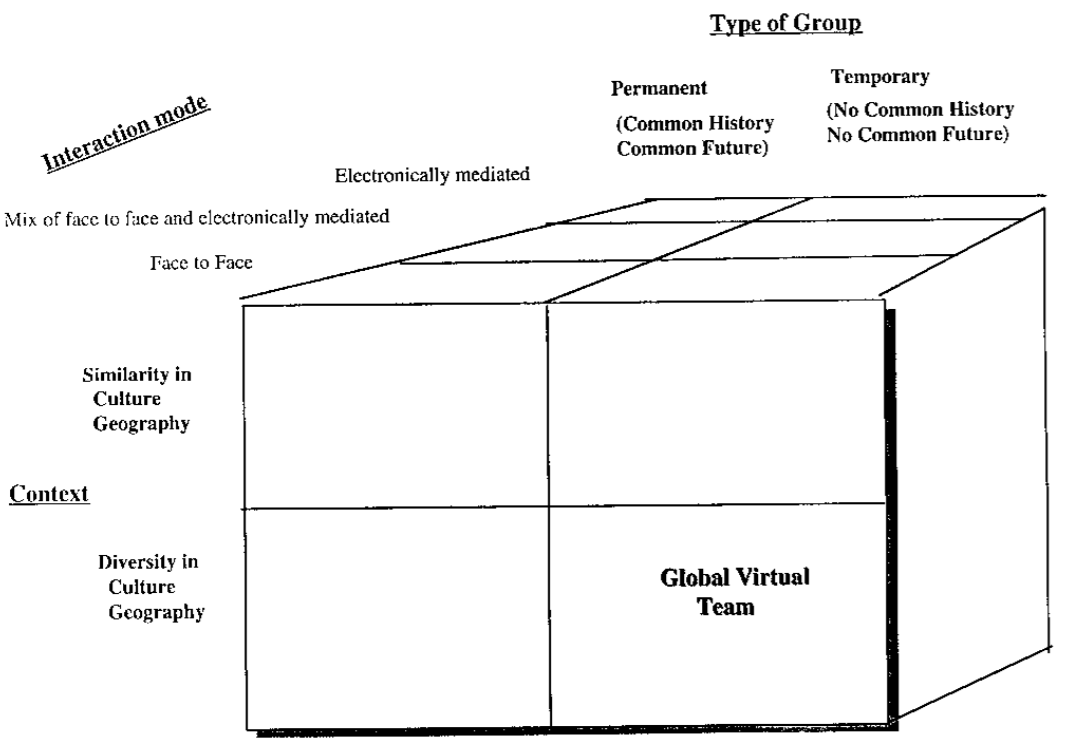
\includegraphics[width=\linewidth]{Abbildungen/GlobalVirtualTeam.PNG}	
			\caption[Virtualität eines virtuellen Teams]{Grad an Virtualität, das ein Team laut Javenpaa et al. \citep{jarvenpaa1999communication} besitzen muss, um als \textit{virtuelles Team} zu gelten.}
			\label{virtualTeamsVirtuality}
		\end{footnotesize}
	\end{figure}

Die Mitglieder eines \textit{virtuellen Teams} haben im Gegensatz zu traditionell geformten Teams weniger Möglichkeiten, sich zu sehen, zu interagieren oder Konflikte zu lösen. 
Respekt und gegenseitiges Verständnis sind die Grundbausteine, um Kreativität und Innovation innerhalb eines Teams zu fördern. Die Effektivität eines Teams ist eine direkte Konsequenz daraus \citep[S. 378]{ren2007applying}.

\paragraph{VIRTUAL TEAMS AND TEAMEFFECTIVENESS}

Wird ein Vergleich zwischen \textit{traditionell} geformten Teams und \textit{virtuellen Teams} gezogen, gehen Schweitzer et al. \citep{schweitzer2010conceptualizing} davon aus, dass traditionell geformte Teams effektiver als \textit{virtuelle Teams} sind und die \textit{Teameffektivität} abnimmt je höher der Grad an Virtualität (siehe \textit{Abbildung \ref{virtualTeamsVirtuality}}) ist.
Diese Meinung teilt auch Becker et al., denn laut ihnen leidet der Austausch des Informationsgehaltes sowie der Vertrauensbildung aufgrund steigender Virtualität und kann nicht dieselbe Effektivität wie ein Face-to-Face Team erreichen \citep{becker2002fuhrung}.

Bisherige Studien haben positive Zusammenhänge \citep{davis2000trusted}, keine Zusammenhänge \citep{hertel2004managing} sowie negative Zusammenhänge \citep{dirks1999effects} zwischen Vertrauen und \textit{Teameffektivität} in \textit{virtuellen Teams} festgestellt.

Trotz der sich widersprechenden Studienergebnisse wird im Allgemeinen die Meinung vertreten, dass Vertrauen einen positiven Einfluss auf die \textit{Teameffektivität} besitzt \citep{de2016trust}. 
Vertrauen in sein Team hilft dabei, eigene Unsicherheiten auszublenden, um sicherer und effektiver arbeiten zu können \citep{de2010does}. Weiterhin entsteht durch vorhandenes Vertrauen in sein Team ein größeres Interesse an den Teammitgliedern, was Synergieeffekte freischaltet und eine direktere und effektivere Interaktion ermöglicht \citep{dirks1999effects}. 

\subsection{AVATARS AND TRUST}
George et al. \citep{george2018trusting} gingen in ihrer Forschung der Frage nach, ob sich in einem Shared-Virtual-Environment mehr Vertrauen zu menschenähnlichen oder roboterartigen Avataren aufbauen lässt und
fanden keinen signifikanten Unterschied in der Vertrauenswürdigkeit. Jedoch wurde ein größeres Gefühl von Gemeinsamkeit festgestellt, wenn mit einem menschenähnlichen Avatar interagiert wurde.

George et al. erwähnten weiterhin in ihrer Studie, dass gute Grafik und realistisches Verhalten durch beispielsweise Mikrogestikulationen und soziale Interaktionen den Aufbau von \textit{Co-Präsenz} unterstützen \citep{george2018trusting}.

Auch Riedl et al. \citep{riedl2014trusting} führte eine Studie zum Vertrauensaufbau unter Menschen im Vergleich zu Avataren mit menschenähnlichen Gesichtern durch. Sie fanden heraus, dass es Personen leichter fällt, einer realen Person, zu vertrauen als einem Avatar mit menschenähnlichem Gesicht. Laut ihnen wird Vertrauen zwischen Menschen in der gleichen Geschwindigkeit aufgebaut wie zwischen Menschen und Avataren.
Diese Vermutung bestätigten auch Bente et al. \citep[S. 54-59]{bente2004social} und stellten fest, dass wenig \textit{kognitives Vertrauen} während der Nutzung des \textit{Shared-Virtual-Environment} zu Avataren aufgebaut werden konnte, während Face-to-Face, Telefon- und Chatkommunikationen besser abschnitten.

\section{METHODS}

Es wurde ein \textit{A/B-Testing} in Kombination mit einem induktiven quantitativen Forschungsdesign gewählt.
Gruppe A bekam dabei die Kondition IK zugeteilt, während Gruppe B die Kondition NIK zugeteilt wurde. Diese Gruppen- und Konditionseinteilung der Teilnehmer erfolgte nach dem Zufallsprinzip. 

Die Analysen dieser Studie wurden auf unterschiedlichen Ebenen durchgeführt.
Da die Teilnehmer als Team arbeiten und unterschiedliche Teams unterschiedliche Konditionen aufweisen, sind einige Zusammenhänge auf \textit{Individualebene}, einige auf \textit{Konditionsebene} und einige auf \textit{Teamebene} zu betrachten.

Die \textbf{Individualebene} sagt etwas über eine einzelne Person aus, während die \textbf{Konditionsebene} zwischen den Konditionen IK und NIK unterscheidet.

Die Konditionsebene kann in einzelne Teams von jeweils 3 Personen aufgeteilt werden. Diese Aufteilung wird als \textbf{Teamebene} bezeichnet und es möglich Aussagen über das Team zu treffen. 
Die \textit{Abbildung \ref{DifferentLevels}} zeigt die Hierarchie der verschiedenen Ebenen.

\begin{figure}[H]
		\begin{footnotesize}
		\centering
			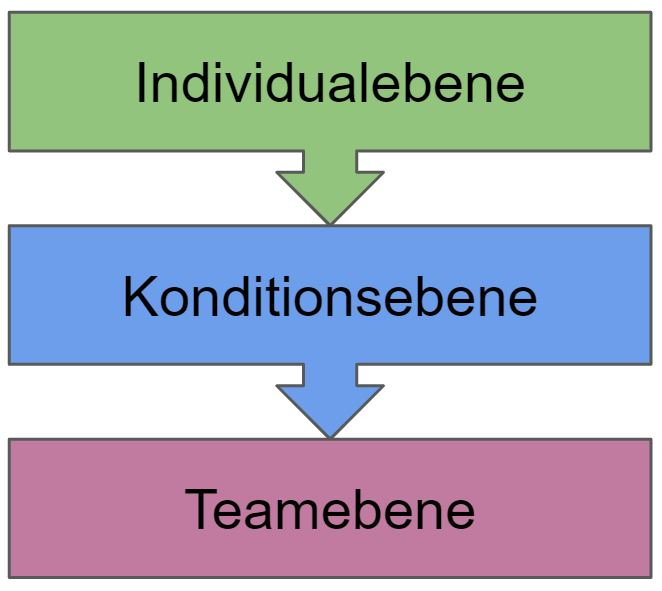
\includegraphics[width=0.5\linewidth]{Abbildungen/DifferentLevels.JPG}	
			\caption[Die Hierarchieebenen]{Die Hierarchie der Individualebene, Konditionsebene und Teamebene.}
			\label{DifferentLevels}
		\end{footnotesize}
	\end{figure}

Anhand eines auf der Theorie basierenden Frameworks (siehe \textit{Abbildung \ref{Versuchshypothesen}}) wurden folgende Hypothesen aufgestellt :

\textbf{H1$_{1}$}: Die Mittelwerte der erzielten \textit{kognitiven Vertrauenswerte} unterscheiden sich bei den Konditionen IK und NIK signifikant voneinander.

\textbf{H2$_{1}$}: Je höher der erzielte \textit{generelle Vertrauenswert} einer Person ist, desto höher ist der erzielte \textit{kognitive Vertrauenswert} einer Person.

\textbf{H3$_{1}$}: Der Zusammenhang zwischen dem \textit{kognitiven Vertrauenswert von Teams} und der \textit{Teameffektivität von Teams} mit der Kondition IK ist stärker als der von Teams mit der Kondition NIK.

\textbf{H4$_{1}$}: Die Mittelwerte der \textit{Teameffektivität} unterscheiden sich bei den Konditionen IK und NIK signifikant voneinander.

\textbf{H5$_{1}$}: Der Zusammenhang zwischen dem \textit{generellen Vertrauenswert eines Teams} und der \textit{Teameffektivität eines Teams} mit der Kondition IK ist stärker als der von Teams mit der Kondition NIK.

\begin{figure}[H]
		\begin{footnotesize}
			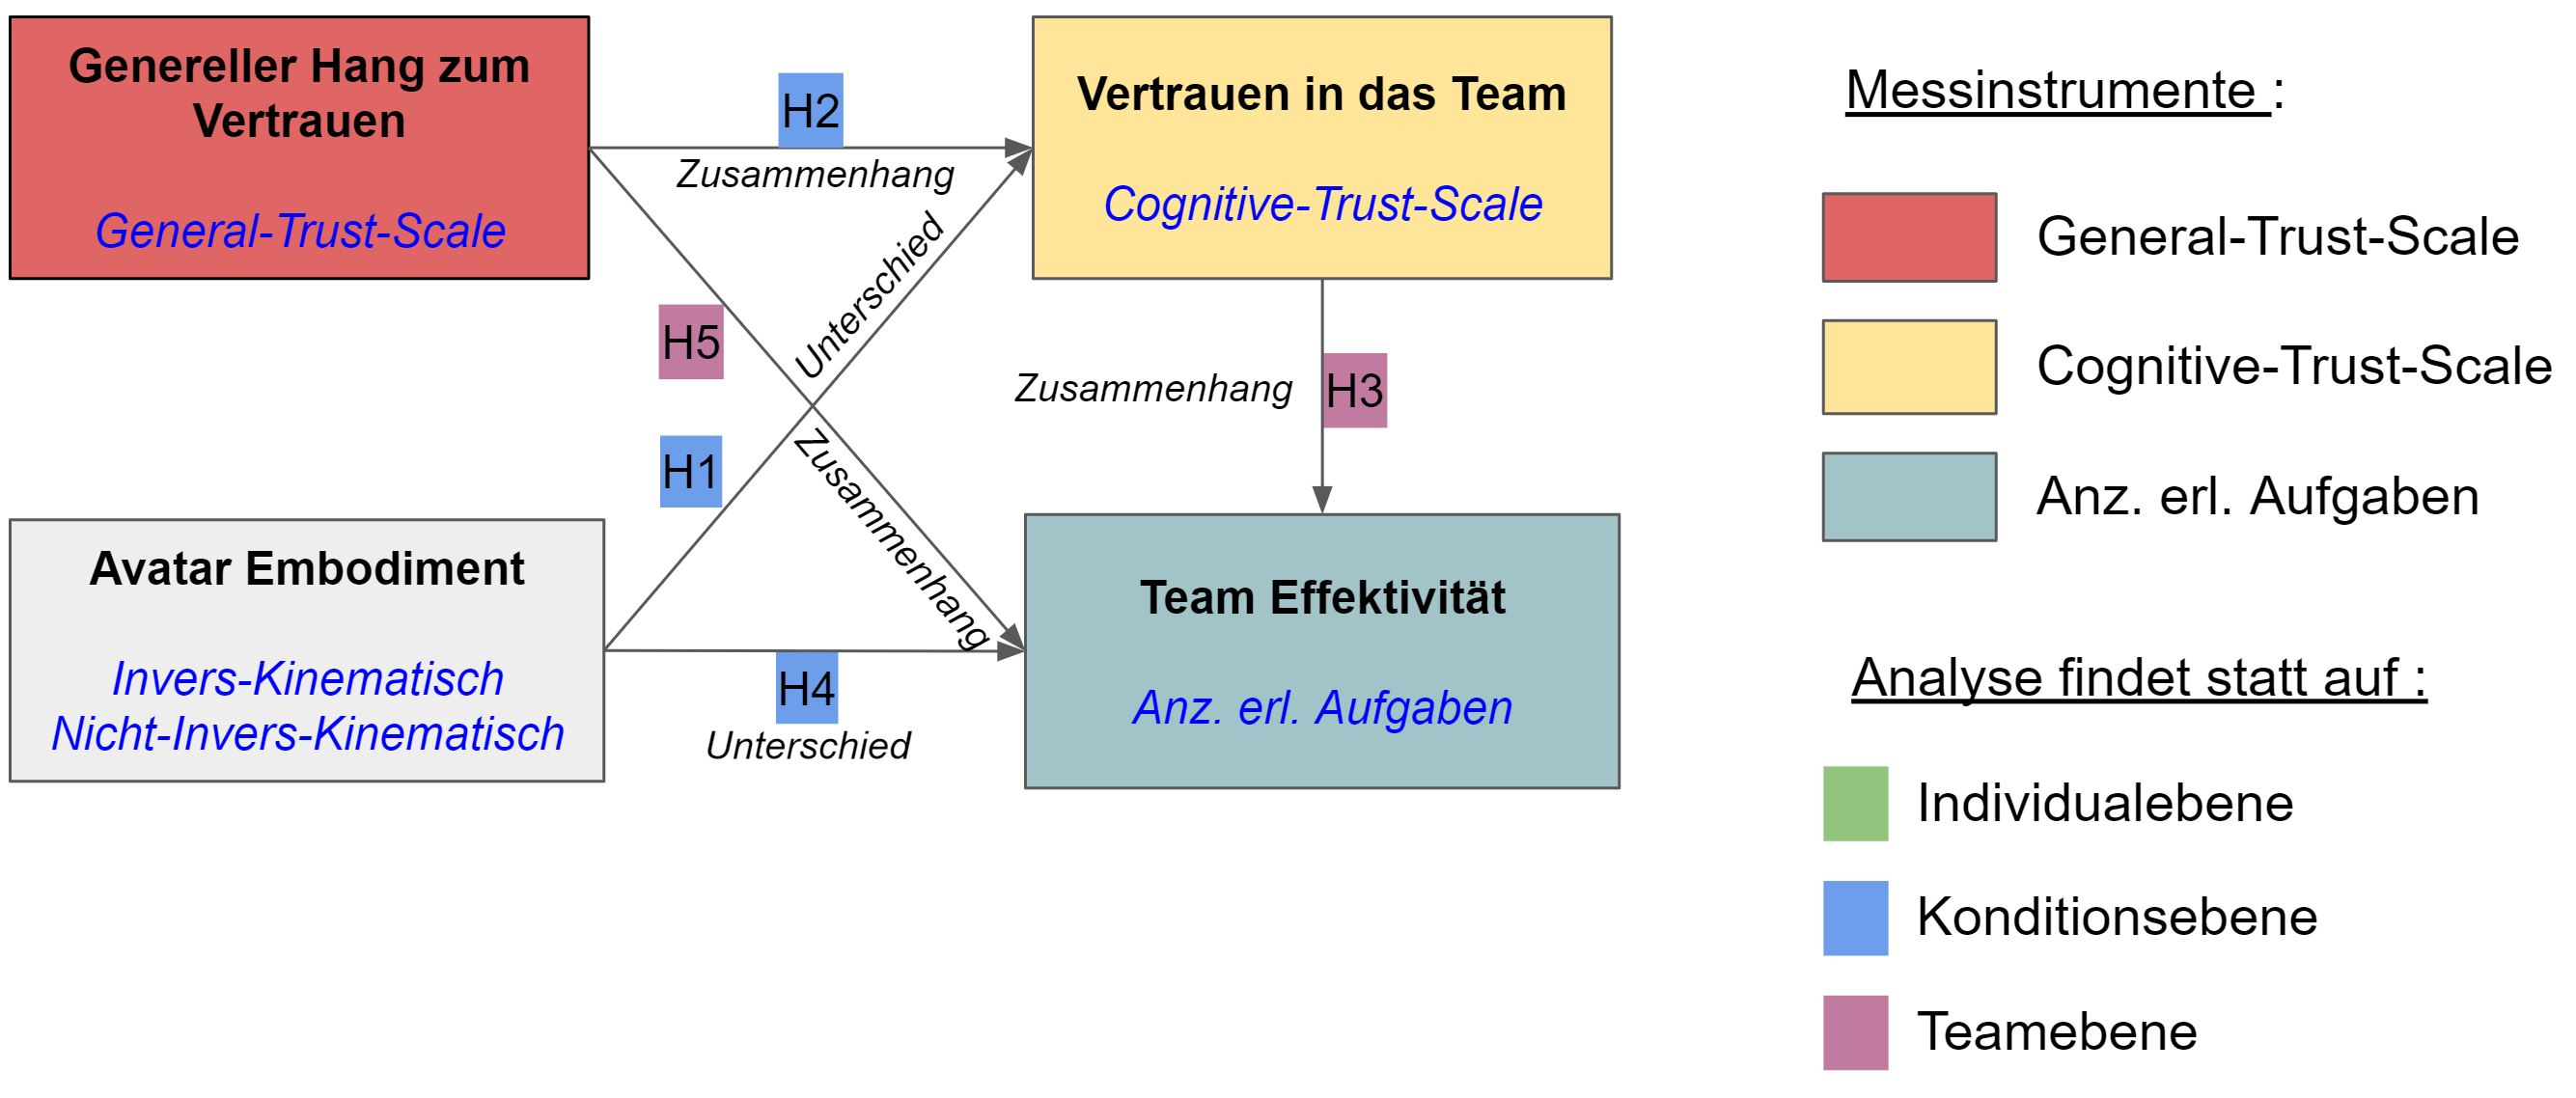
\includegraphics[width=\linewidth]{Abbildungen/Versuchshypothesen_02.JPG}		
			\caption[Das Framework der Versuchshypothesen]{Dieses Framework verdeutlicht, wie die Hypothesen zusammenhängen.}
			\label{Versuchshypothesen}
		\end{footnotesize}
	\end{figure}	

Das generelle Vertrauen bezieht sich in dieser Studie darauf, wie sehr die Teilnehmer dazu neigen, anderen Personen einen Vertrauensvorschuss zu gewähren. \citep[S. 30]{mcallister1995affect}.
Das \textit{kognitive Vertrauen} bezieht sich auf die \textit{Überzeugung in die Fähigkeiten oder in die Zuverlässigkeit eines anderen} \citep[S. 30]{mcallister1995affect}.
Die \textit{Teameffektivität} wird anhand der Anzahl der abgeschlossenen Runden des Teams während des Experiments gemessen.

\subsection{MEASURING METHODS}
Der General-Trust-Scale ($\alpha =,91$) \citep{couch1996assessment} wurde eingesetzt, um den generellen Vertrauenswert der einzelnen Teilnehmer zu messen. 

Der Cognitive-Trust-Scale ($\alpha =,91$) Fragebogen ist ein Auszug des von McAllister et al. \citep[S. 37]{mcallister1995affect} entwickelten Fragebogens. Er überprüft, wie viel \textit{kognitives Vertrauen} die Teilnehmer während des Versuchs aufbauen.

Gonzales-Rom et al. \citep[S. 1049]{gonzalez2014climate} entwickelten 2004 einen Fragebogen, um die \textit{Qualität von Teamkommunikation} ($\alpha =,76$) zu messen.

Gibson et al. \citep[S. 469]{gibson2003team} entwickelten 2003 einen Fragebogen, der die \textit{wahrgenommene Teameffektivität} ($\alpha =,62-,88$) misst. In dieser Studie wurde ein Auszug des Fragebogens verwendet. Er misst das \textit{subjektive Ausmaß der wahrgenommenen Teameffektivität}.

Der NASA-TLX ($\alpha =,84$) erfragt die allgemeine Belastung der Probanden, die sie während des Experiments empfunden haben. 

Der IPQ ($\alpha =,85$) dient zur \textit{Messung des Präsenz-Gefühls} in einer virtuellen Umgebung. Er misst, inwieweit sich der Nutzer in der virtuellen Umgebung anwesend fühlt, inwieweit der Nutzer seine Aufmerksamkeit der virtuellen Umgebung schenkt und wie real die virtuelle Umgebung dem Nutzer erschien. 

Mithilfe des \textit{Co-Präsenz-Fragebogens} können die \textit{selbst gemeldete Co-Präsenz} ($\alpha =,78$), die \textit{wahrgenommene Präsenz des anderen} ($\alpha =,90$), die \textit{Telepräsenz} ($\alpha =,88$) sowie die \textit{soziale Präsenz} ($\alpha =,82$) ermittelt werden.
\subsection{PARTICIPANTS}

The participants were acquired in two ways. On the one hand, people in the circle of acquaintances were approached, who would be provided with the necessary hardware. Secondly, participants were sought in various forums (e.g. VRForum.de, Computerbase.de, Hardwareluxx.de, etc.). Furthermore, participants were acquired with the help of various social networks related to VR as well as random WhatsApp chat groups with 50 or more members.

To participate in the experiment, participants needed a fully functioning SteamVR, Windows Mixed Reality, or Oculus Rift/Rift-S head-mounted display with compatible controllers, as well as a powerful VR-enabled PC. The experimenter used a PC without a head-mounted display to control and manage the experiment from outside.

\subsection{PROCEDURE AND IMPLEMENTATION}
Um den Versuch durchzuführen, wurde ein Shared-Virtual-Environment entwickelt, in dem sich die drei Teammitglieder gegenseitig als Avatare sehen und miteinander interagieren können. Das Shared-Virtual-Environment ist mit Unity 2019.4.3f1 und der HD-Render-Pipeline entwickelt worden. Um die Echtzeitkommunikation zwischen den einzelnen Clients zu gewährleisten, wurde das Multiplayer-Framework \textit{Normcore v2.0}\footnote{www.Normcore.io} genutzt.

Es sind jeweils drei Personen in einem Zeitslot untergebracht worden, um ein Team zu bilden. Die Teilnehmer wurden untereinander \textit{nicht} Face-to-Face vorgestellt und sahen sich nur als Repräsentation eines Avatars.
Der Versuch dauerte 35 Minuten und teilte sich auf in
		\begin{itemize}
			\item 5 Minuten Pre-Questionnaire,
			\item 5 Minuten Videoerklärung,
			\item 10 Minuten Versuchsdurchführung,
			\item 15 Minuten Post-Questionnaire.
		\end{itemize}
Der Pre-Questionnaire diente dazu, allgemeine Demografische Daten der Teilnehmer zu erfahren. Das Erklärvideo zeigt alle relevanten Mechaniken und Funktionsweisen. Weiterhin wurde sichergestellt, dass alle teilnehmende Person denselben Informationsgehalt über die Art und Weise des Ablaufs des Experiments besaßen. Während der Versuchsdurchführung hatten die Teilnehmer 10 Minuten Zeit, möglichst viele Runden im Team zu absolvieren. Über den anschließenden Post-Questionnaire wurden alle relevanten Fragebögen abgefragt. Die maximale Versuchsdauer nach Start der Anwendung betrug exakt 600 Sekunden) und es konnten maximal 15 Runden absolviert werden. Die Runden wurden in jeder dritten Runde inrekmentell schwieriger da jeweils ein Symbol in den Pool der zu erratenden Symbole hinzukam.
 \textit{Abbildung \ref{RoundDifficulty}} zeigt die steigenden Schwierigkeitswerte, anhand derer in diesem Experiment die \textit{Teameffektivität} gemessen wurde.

\begin{figure}[H]
		\begin{footnotesize}
		\centering
			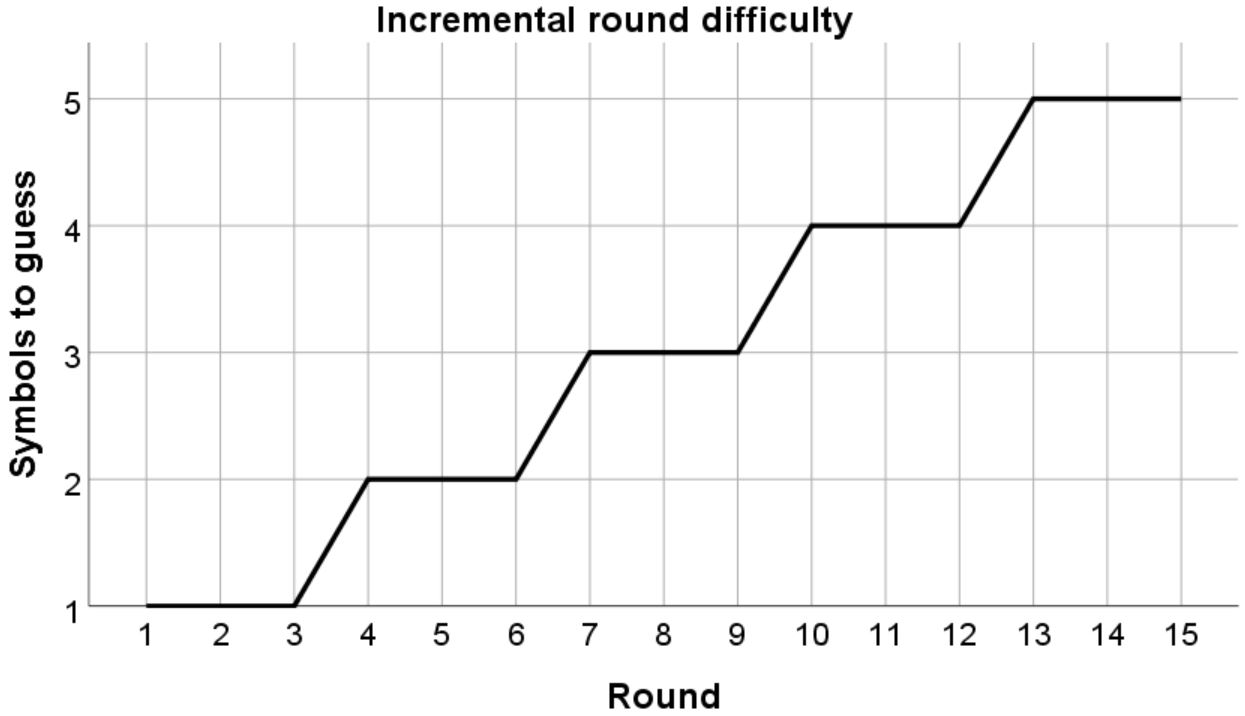
\includegraphics[width=0.7\linewidth]{Abbildungen/RoundDifficulty.JPG}	
			\caption[Der Schwierigkeitsgrad der Runden]{Die steigende Schwierigkeit der zu erratenden Symbole der einzelnen Runden. In Runde 1-3 muss ein Symbol erraten werden, in Runde 3-6 zwei Symbole usw.}
			\label{RoundDifficulty}
		\end{footnotesize}
	\end{figure}

Zu Beginn jeder neuen Runde konnten die Spieler die Zuteilung der Farben sehen und dadurch den Startspieler identifizieren. Dieser ist schwarz markiert und hat die Aufgabe, seinen Mitspielern die für ihn farblich gekennzeichneten Symbole zu erklären. Seine Mitspieler mussten die ihnen zugeteilten Symbole identifizieren und an ihrem Podest einloggen. Das Ziel war, so viele Symbole wie möglich individuell korrekt zu erkennen, um dadurch gemeinsam in höhere Runden aufzusteigen.

Die Symbole auf dem Podest des schwarz markierten Spielers wurden entweder durch die Farbe Grün, Rot oder Grün-Rot gekennzeichnet. Auf den Podesten der Mitspieler befanden sich ebenfalls Symbole, welche jedoch zufällig angeordnet sind und keine farblichen Markierungen hatten. Der schwarz markierte Spieler versuchte nun, mittels Hand- und Armbewegung, den rot und grün markierten Mitspielern die Symbole, die in der jeweiligen Spielerfarbe vor ihm markiert waren, zu erklären. Meinte der gerade angesprochene Mitspieler ein Symbol erkannt zu haben, loggte dieser das Symbol durch das Herunterdrücken des passenden Knopfes an seinem Podest ein. 

Wurden alle gekennzeichneten Symbole vom roten und grünen Spieler erkannt und eingeloggt, erschien eine leuchtend grüne Kugel, die das Ende einer Runde anzeigte. Erschien diese grüne Kugel nicht, war noch ein Symbol falsch eingeloggt und der schwarz markierte Spieler musste noch einmal versuchen, die korrekten Symbole den jeweiligen Mitspielern aufzuzeigen. 
In der nächsten Runde war ein anderer Spieler eindeutig mit Schwarz, Rot oder Grün markiert.
In der folgenden Runde erhielt jeder Spieler wieder eine andere der drei Farben.
\textit{Abbildung \ref{AvatareImEinsatz}} zeigt beide Avatar-Konditionen IK (a) und NIK (b) während der Versuchsdurchführung im Spectatorview.
	
\begin{figure}[h]
  \centering
  \subfloat[][]{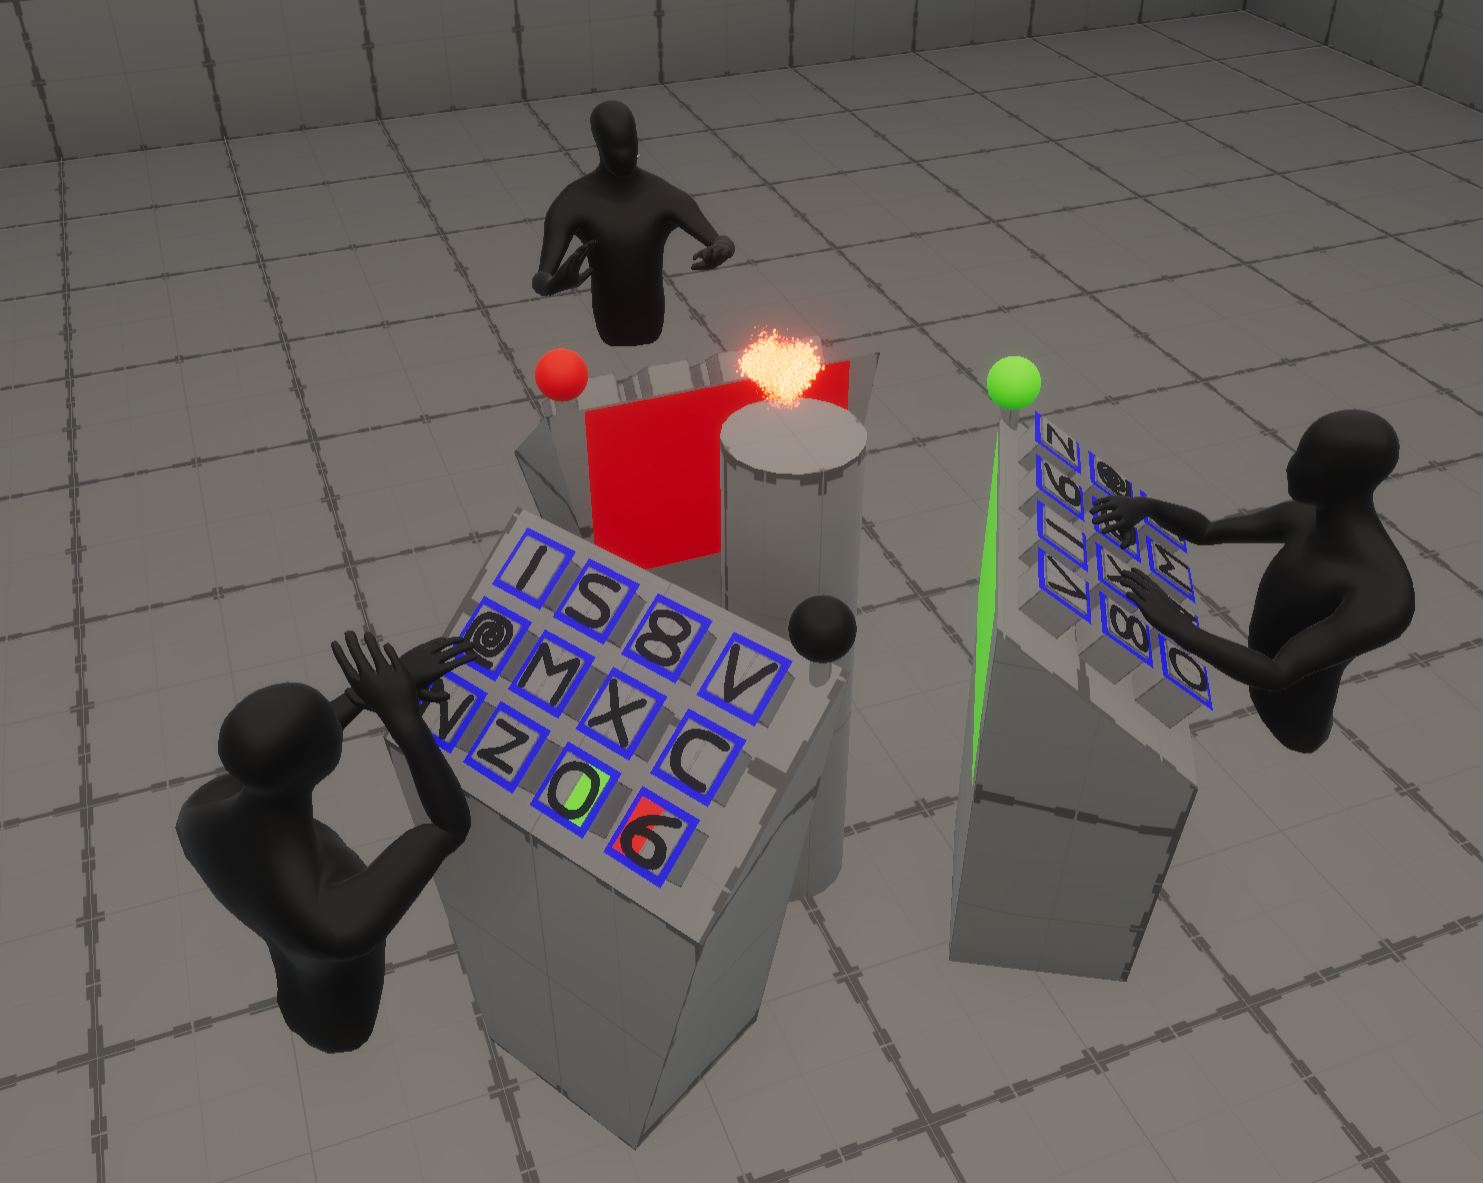
\includegraphics[width=0.45\linewidth]{Abbildungen/Podeste_IK_Avatars.jpg}}
  \qquad
  \subfloat[][]{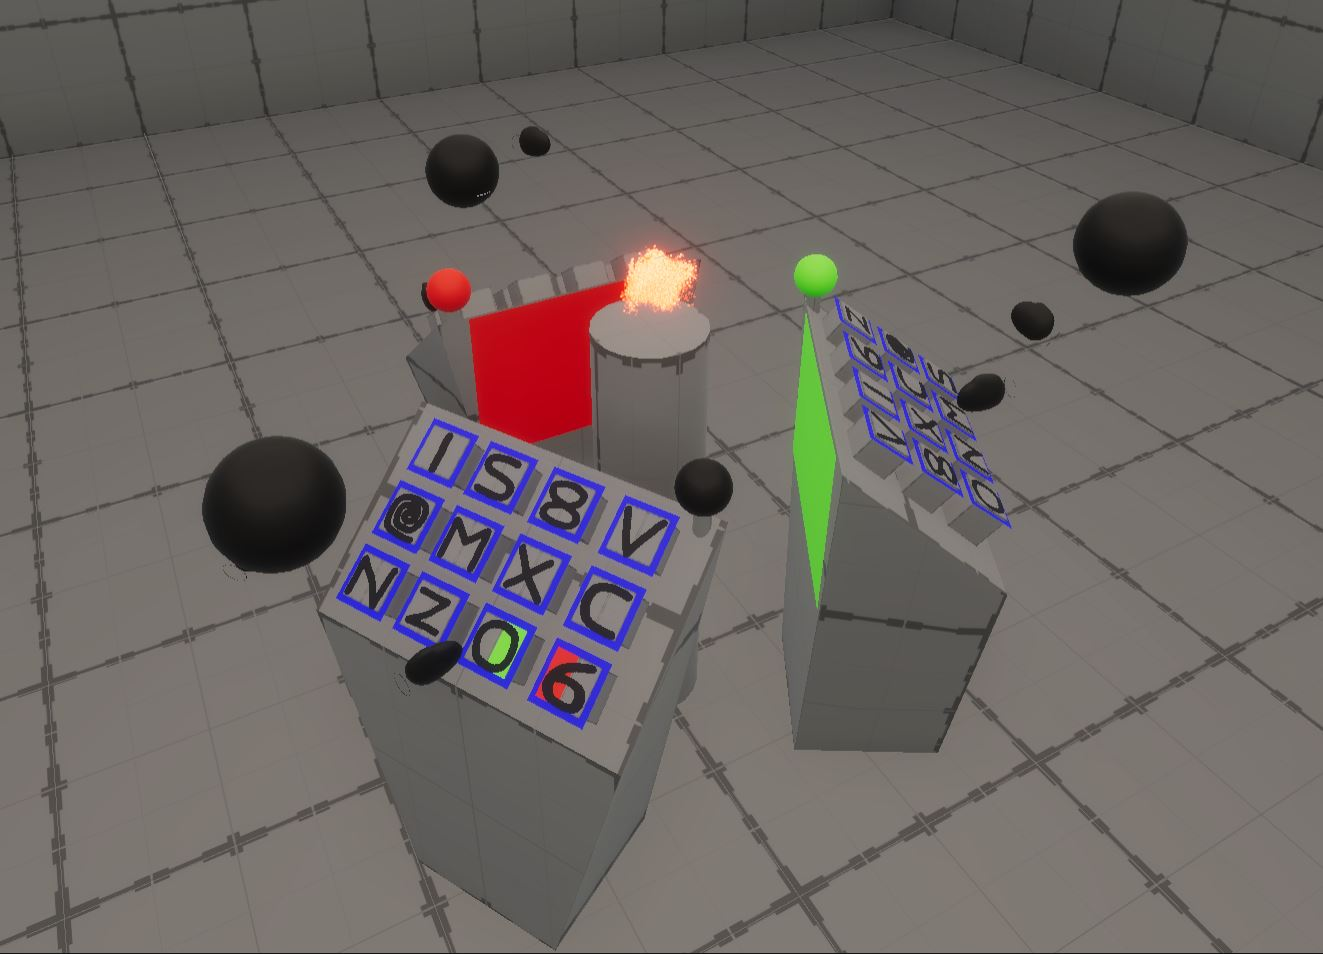
\includegraphics[width=0.45\linewidth]{Abbildungen/Podeste_Non_IK_Avatars.jpg}}
  \qquad
  \subfloat[][]{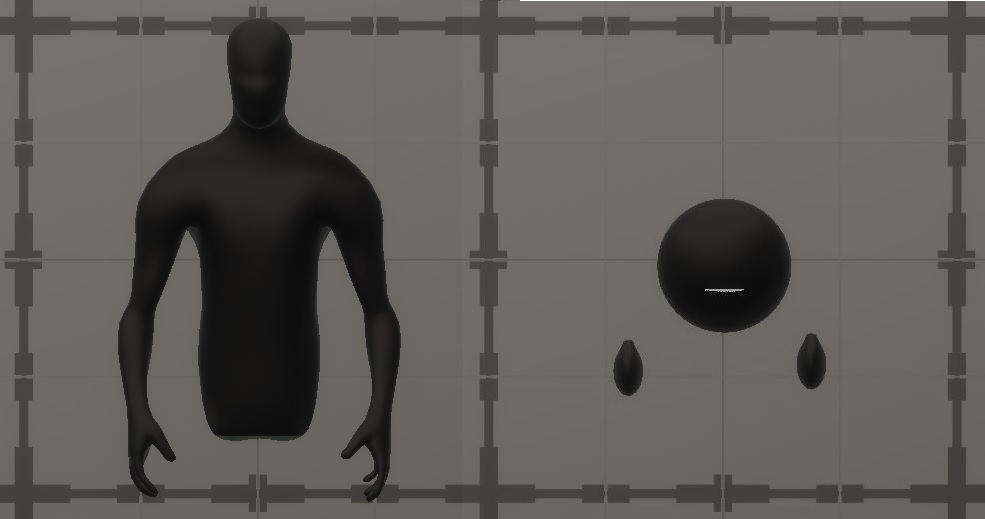
\includegraphics[width=0.45\linewidth]{Abbildungen/Avatars.JPG}}
  \caption[Die Avatare und der Spectatorview]{Avatar-Konditionen IK (a) und NIK (b) während der Versuchsdurchführung im Spectatorview. (c) zeigt die verwendeten Avatare nebeneinander. Links: IK-Avatar und rechts: Non-IK-Avatar.}
  \label{AvatareImEinsatz}
\end{figure}

\section{RESULTS}
\subsection{HYPOTHESIS}
%H1
Anhand der statistischen Analyse der Hypothese 1 lässt sich feststellen, dass unterschiedliche Avatar-Konditionen einen \textit{signifikanten} Einfluss auf das gebildete \textit{kognitive Vertrauen} besitzen (Mann-Whitney-U $U = 64,000; Z = -2,029; p =,042 < \alpha =,05; r =-,370$). Dabei haben Teilnehmer mit der Kondition NIK $(\bar{x} = 4,622)$ mehr \textit{kognitives Vertrauen gebildet} als Teilnehmer mit der Kondition IK $(\bar{x} = 4,188)$. 

%H2
Durch die Analyse der Hypothese 2 \textit{keine Anzeichen} dafür, dass es einen \textit{signifikanten} Zusammenhang zwischen dem \textit{generellen Vertrauen} und dem \textit{kognitiven Vertrauen} besteht. 

%H3
Entgegen der Annahme der \textit{Hypothese 3} wurde ein \textit{signifikanter} Zusammenhang zwischen dem gebildeten \textit{kognitiven Vertrauen im Team} und der \textit{Teameffektivität} bei der Kondition NIK festgestellt (Spearman-Rho $r =,975$; $p =,005 < \alpha = ,05$). Dieser Zusammenhang unterscheidet sich laut Fisher-Z-Wert für unabhängige Stichproben ($Z=-1.977$), \textbf{signifikant} ($p =,024 < \alpha = ,05$) von dem der Kondition IK.
 
%H4
Es wurde während der Analyse der Hypothese 4 festgestellt, dass sich die \textit{Teameffektivität} aufgrund von unterschiedlichen Avatarkonditionen \textit{nicht signifikant} voneinander unterscheidet (Mann-Whitney-U $U = 103,500; Z = -,377; p =,706 > \alpha = ,05; r = -,060$). Bei beiden Avatarkonditionen wurde eine durchschnittliche Teameffektivität von $\bar(x) = 9$ festgestellt.

%H5
Weiterhin gibt es aufgrund der Analyse der Hypothese 5 \textit{keine Anzeichen} dafür, dass es einen \textit{signifikanten} Zusammenhang zwischen dem \textit{generellen Vertrauen} einer Person \textit{Teameffektivität} in einem \textit{virtuellen Team} gibt.

Es wurde ein \textit{signifikanter} Unterschied der Mittelwerte der Teamkommunikation auf Konditionsebene festgestellt. Zudem kann festgehalten werden, dass sich ein erhöhtes Präsenz-Gefühl (Präsenz, Telepräsenz, selbst wahrgenommene Co-Präsenz, wahrgenommene Co-Präsenz des anderen und Soziale-Präsenz) auf Konditionsebene während der Versuchsdurchführung gebildet hat. Die allgemeine Belastung lag unter dem Durchschnitt der möglichen anzugebenden Werte und die wahrgenommene Teameffektivität war überdurchschnittlich hoch.
Weiterhin gibt es einen \textit{signifikant} positiven Zusammenhang zwischen dem \textit{kognitiven Vertrauen} und der \textit{wahrgenommenen Teameffektivität}  (Spearman-Rho : ($r =,869; p =,000 < \alpha = ,05$) und der \textit{Teamkommunikation} ($r =,676; p =,006 < \alpha = ,05$) auf Konditionsebene bei der Kondition NIK.

\subsection{SUBJECTIVE DATA}
Anhand eines Mann-Whitney-U-Test konnte bei der Kategorie \textit{Teamkommunikation} ein \textit{signifikanter Unterschied} zwischen den Mittelwerten beider Avatar-Konditionen festgestellt werden (Mann-Whitney-U : $U = 63,500; Z = -2,062; p =,039 < \alpha = ,05$). Der Mittelwert der \textit{Teamkommunikation} der Kondition IK beträgt $\bar{x} = 4.013$, während der Mittelwert der Teamkommunikation der Kondition NIK $\bar{x} = 4,48$ beträgt. Somit ist die subjektiv empfundene Teamkommunikation bei der Kondition NIK signifikant höher als bei der Kondition IK und bei beiden Konditionen ist die Tendenz einer hohen Teamkommunikation ersichtlich ($\bar{x} = 4,013$; $\bar{x} = 4,48$ $ > \bar{x}  = 3$).

Das von allen Teilnehmern durchschnittlich angegebene \textit{Gefühl der Präsenz} kann mit dem Wert $\bar{x} = 4,446$ als stark interpretiert werden ($\bar{x} > 3,5$). Die \textit{Telepräsenz} ($\bar{x} = 5,286$) sowie die \textit{soziale Präsenz} ($\bar{x} > 6,409$) werden etwas stärker als durchschnittlich empfunden und deuten dadurch auf ein höheres Gefühl der Anwesenheit sowie auf ein stärkeres Gefühl der Nähe zwischen den Teilnehmern hin. Auch die \textit{selbst wahrgenommene Co-Präsenz} sowie die \textit{wahrgenommene Co-Präsenz des anderen} liegen mit den Werten $\bar{x} = 3,827$ und $\bar{x} = 3,877$ über dem Mittelwert der Antwortmöglichkeiten ($\bar{x} > 2,5$) und weisen somit eine Tendenz zur starken \textit{Co-Präsenz} auf.

Daneben liegt die durchschnittlich \textit{wahrgenommene Teameffektivität} mit dem Wert $\bar{x} > 4,886$ über dem Wert 3,5 und lässt sich somit im Bereich der als eher stark empfundenen Teameffektivität ($3,5 - 7$) verorten.
Die Werte des NASA-TLX (Allg. Anstrengung) ($\bar{x} < 7$) zeigen, dass das VR Experiment als mittelmäßig bis wenig anstrengend wahrgenommen wurde ($\bar{x} < 11$ ).

Auf Konditionsebene ist eine signifikante ($r =,869; p =,000 < \alpha = ,05$) starke positive Korrelation (vgl. \citep{cohen2013statistical}) mit dem Spearman- Korrelationskoeffizient  zwischen den \textit{kognitiven Vertrauenswerten} und \textit{der wahrgenommenen Teameffektivität} der Kondition NIK zu erkennen.

Weiterhin ist eine signifikante ($r =,676; p =,006 < \alpha = ,05$) positive Korrelation starken Effektes (vgl. \citep{cohen2013statistical}) zwischen den \textit{kognitiven Vertrauenswerten} und der \textit{Team-Kommunikation} der Kondition NIK auf Konditionsebene zu erkennen.

\section{DISCUSSION}
\subsection{Building trust through the avatar conditions}
Die Ergebnisse des Experiments widersprechen der Untersuchung von Bente et al. (vgl. Kapitel \ref{AvatarTrust}), die vermuten ließ, dass bei der Kondition IK ein größerer \textit{kognitiver Vertrauensaufbau} stattfindet als bei der Kondition NIK (Hypothese 1). Es ist laut der statistischen Auswertung genau das Gegenteil der Fall, denn die Teilnehmer mit der Kondition NIK erzielen im Durchschnitt einen signifikant höheren kognitiven Vertrauenswert.
Ein Grund für dieses Ergebnis könnte sein, dass der verwendete IK-Avatar vom \textit{Uncanny Valley Effekt} \footnote{Der Uncanny-Valley Effekt beschreibt das Gefühl des Unbehagens ab einem gewissen Realitätsgrad  \citep[S. 352-353]{gast2011unheimliche}.} betroffen ist.
Weiterhin könnte die in diesem Experiment verwendete Inverse-Kinematik, als fremdartig empfunden worden sein. Auch dadurch falsch interpretierte Gestikulation kann zu einem geringeren Vertrauensaufbau in das jeweilige Gegenüber geführt haben.

\subsection{Building trust through the general trust}
Dass kein signifikanter Zusammenhang zwischen dem \textit{kognitiven Vertrauen} und dem \textit{generellen Vertrauen} bei unterschiedlichen Avatar- Konditionen besteht (Hypothese 2), kann auch als Vorteil gesehen werden.
So lässt sich vermuten, dass es während einer kurzfristigen Zusammenarbeit in einem Shared-Virtual-Environment nicht von Relevanz ist, wie hoch oder niedrig das \textit{generelle Vertrauen} einer Person ist. 
Da nur die unterschiedlichen Avatar-Konditionen einen signifikanten Einfluss auf die Bildung des kognitiven Vertrauens besitzen, kann davon ausgegangen werden, dass das \textit{generelle Vertrauen} während einer Kennenlernphase eines virtuellen Teams keine größere Rolle spielt und isoliert betrachtet werden kann.

\subsection{Trust in the team and team effectiveness}
Die Hypothese 3, in der vermutet wurde, dass der Avatar mit der Kondition IK mehr \textit{kognitives Vertrauen} aufbaut, muss ebenfalls abgelehnt werden. Jedoch wurde während der Analyse dieser Hypothese festgestellt, dass es einen \textit{signifikanten Zusammenhang} zwischen dem gebildeten \textit{kognitiven Vertrauen} und der \textit{Teameffektivität} der Kondition NIK gibt. Da die Hypothese 4 nicht angenommen werden kann, jedoch ein signifikanter Zusammenhang mit der Kondition NIK bei der Analyse der Hypothese 3 festgestellt wurde, muss vermutet werden, dass die Ergebnisse der Hypothese 3 und Hypothese 4 entweder zufälliger Natur sind oder die Messung der Teameffektivität verbessert werden muss.
Die kleine Stichprobengröße der Studie könnte zudem eine Ursache dafür sein, dass die Ergebnisse von Hypothese 3 und Hypothese 4 keine eindeutigen Ergebnisse liefern. Bei einer deutlich größeren Stichprobengröße könnte bei einer größeren Varianz der \textit{Teameffektivitätswerte} gegebenenfalls ein signifikanter Unterschied oder ein eindeutiger signifikanter Zusammenhang mit dem \textit{kognitiven Vertrauen} und der \textit{Teameffektivitätswerte}, festgestellt werden.

\subsection{LIMITATIONS}
Als technische Limitation dieser Arbeit kann die eingesetzte Technik der Gestikulation aufgeführt werden. Die unterstützten Head-Mounted-Displays boten keine Möglichkeit, die Finger oder die gesamten Hände in der Virtual-Reality abzubilden. Die Verständigung innerhalb des Shared-Virtual-Environment kann durch den Einsatz von Finger- und Handtracking intensiviert werden, da verschiedene Gesten genauer wiedergegeben werden können. Das Finger- und Handtracking ist beispielsweise durch eine Oculus Quest oder Oculus Quest 2 möglich. Ein weiterer Aspekt, um die Menschenähnlichkeit und den Realismus bei der Avatar-Kondition IK zu erhöhen, wäre der Einsatz von Mimik.
Eine weitere Limitierung dieser Untersuchung war, dass die Teilnehmer bevor das Experiment startete wussten, dass diese in einem Shared-Virtual-Environment mit realen Personen agieren würden. 
Darüber hinaus ist der Avatar mit der Kondition IK in dieser Studie nicht auf Menschenähnlichkeit, Realismus oder Ähnliches überprüft worden. 
\section{CONCLUSION AND FUTURE WORK}
Shared-Virtual-Environments entwickeln sich aktuell sehr rasant. Die Coronapandemie hat gezeigt, dass virtuelle Kollaborationsmaßnahmen einen großen Einfluss auf Unternehmen weltweit haben. Es ist mehr Forschung darüber nötig, wie Teams effektiv in einem Shared-Virtual-Environment zusammenarbeiten können.

Es könnte nicht nur untersucht werden, welche Art eines Avatars in einem Shared-Virtual-Environment mehr Vertrauen schafft oder mehr \textit{Teameffektivität} erzeugt, sondern auch, wie die eingesetzte Sprache, die Mimik, die Gestik, die Größe, das Geschlecht oder der vorherige Bekanntheitsgrad der Personen sich auf das Vertrauen und die \textit{Teameffektivität} auswirkt.
Weiterhin könnte untersucht werden, wie die Art und Dauer der Nutzung des Head-Mounted-Displays, während ein Team zusammenarbeitet, sich auf das Vertrauen ins Team und die Teameffektivität auswirkt.

Eine Weiterführung dieser Studie könnte untersuchen, in welchem Maß sich der \textit{kognitive Vertrauensaufbau im Team} ändert, je nachdem, ob die Teilnehmer wissen, dass sie mit Menschen zusammenarbeiten oder nicht. Darüber hinaus wäre es interessant zu untersuchen, wie sehr sich der Unterschied zwischen einer verbalen und einer nonverbalen Kommunikation auf das gebildete Vertrauen im Team in einem Shared-Virtual-Environment auswirkt.  
Weiterhin könnten ähnliche Studien durchgeführt werden, bei denen die einzelnen Runden der Kollaborationsaufgabe schneller hintereinander ausgeführt werden oder die Avatare ein anderes Aussehen besitzen.

Es konnte ein signifikanter Unterschied beim gebildeten \textit{kognitiven Vertrauen} zwischen den Avatar-Konditionen festgestellt werden, wobei sich mehr \textit{kognitives Vertrauen} bei den nicht- menschenähnlichen Avataren bildete. Es konnte jedoch kein statistisch signifikanter Unterschied zwischen den Avatar-Konditionen und der \textit{Teameffektivität} festgestellt werden. Weiterhin zeigen die Ergebnisse keinen signifikanten Zusammenhang zwischen dem \textit{generellen Vertrauen} und dem gebildeten \textit{kognitiven Vertrauen} einer Person. Zwischen dem \textit{kognitiven Vertrauen} und der \textit{Effektivität eines Teams} konnte ein signifikanter Zusammenhang bei der Kondition IK festgestellt werden.

In einem virtuellen Team besitzt die Avatar-Kondition laut dieser Studie somit keinen eindeutigen Einfluss auf die \textit{Teameffektivität}. Es kann jedoch sinnvoll sein, den Avatar nicht zu menschenähnlich zu gestalten, um mehr \textit{kognitives Vertrauen} zu bilden.
%Es empfiehlt sich, diese Studie mit einer großen Stichprobe zu replizieren und die Einflüsse anders gestalteter Avatare zu untersuchen. 
Die Arbeit in einem virtuellen Team muss folglich nicht mit aufwendig gestalteten Avataren unterstützt werden. So können beispielsweise Unternehmen, die mit virtuellen Teams in einem Shared-Virtual-Environment arbeiten wollen, auf simple Avatar-Modelle zurückgreifen, um den Vertrauensaufbau im Team zu unterstützen.

%%
%% The next two lines define the bibliography style to be used, and
%% the bibliography file.
%\citestyle{acmauthoryear}
\bibliographystyle{ACM-Reference-Format}

\bibliography{sample-base}

%%
%% If your work has an appendix, this is the place to put it.
\appendix


\end{document}
\endinput
%%
%% End of file `sample-sigconf.tex'.
